%%%%%%%%%%%%%%%%%%%%%%%%%%%%%%%%%%%%%%%%%%%%%%%%%%%%%%%%%%%%%%%%%%%%%%%%%%%%%%%
%                                    __  _                ___                 %
%                    ________  _____/ /_(_)___  ____     <  /                 %
%                   / ___/ _ \/ ___/ __/ / __ \/ __ \    / /                  %
%                  (__  )  __/ /__/ /_/ / /_/ / / / /   / /                   %
%                 /____/\___/\___/\__/_/\____/_/ /_/   /_/                    %
%                                                                             %
%%%%%%%%%%%%%%%%%%%%%%%%%%%%%%%%%%%%%%%%%%%%%%%%%%%%%%%%%%%%%%%%%%%%%%%%%%%%%%%

\section{(1)}
  \subsection{1990年代の後半からレーザーのピーク出力の増大に貢献した技術}
    図\ref{Laser_intensity_vs_years}から1990年代の後半からレーザーのピーク出力の増大に
    貢献した技術として, CPA(チャープパルス増幅)法が考えられます。CPAは1985年にロチェスター
    大学のレーザー物理学者であるRochester StricklandとMourou(1985)、
    MaineとMourou(1988)、Maineら(1988)によって実証されました。\cite{ref. 01}
    \begin{figure}[H]
      \centering
      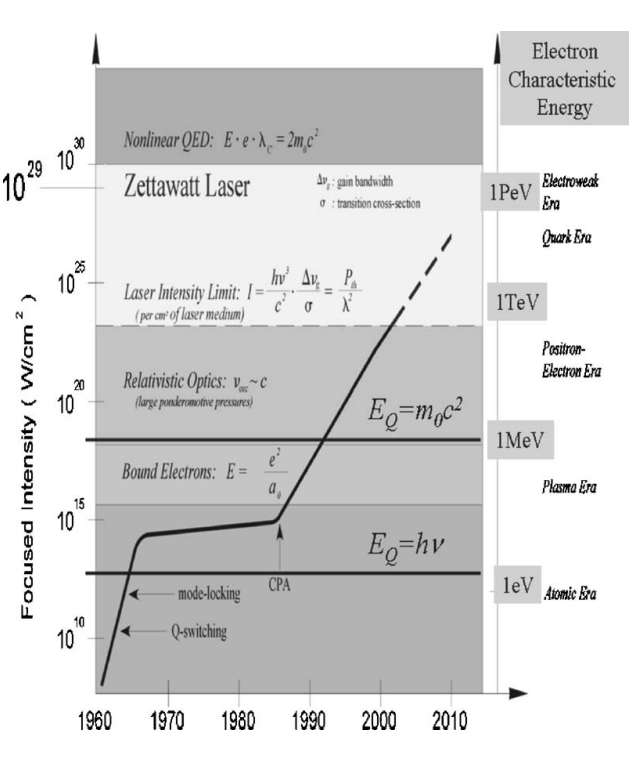
\includegraphics[width=0.42\textwidth]{
        \ONE/laser_intensity_vs_years.png
      }
      \caption{Laser intensity vs years \\ G. A. Mourou and T. Tajima. Rev. Mod. Phys. \bm{78}, 309 (2006).}
      \label{Laser_intensity_vs_years}
    \end{figure}

  \subsection{チャープパルス増幅}
    \subsubsection{チャープパルス増幅の原理}
      まず、短く低エネルギーのパルスを単一モード光ファイバー内で意図的に伸張させて長いパルスを
      生成します。パルスは、群速度分散と自己位相変調の組み合わせによってファイバー内で線形チャ
      ープがかかります。伸張されたパルスは増幅され、その後、二重回折格子コンプレッサーによって
      圧縮されます。伸張されたパルスを増幅することで、自己集束が発生する前により高いエネルギー
      を達成することが可能になります。この増幅はチャープの線形性に影響を与えないため、パルスは
      完全に圧縮されます。不均質な媒質でチャープパルスを増幅することの潜在的な利点として、利得
      掃引が挙げられます。この場合、パルス幅に沿って周波数が変化するため、増幅されたパルスは利
      得飽和の影響を受けず、各周波数成分が独立して利得を得られます。\cite{ref. 02}

    \subsection{チャープパルス増幅が現在のレーザー技術やレーザーの応用技術にもたらした意義、波及効果}
      CPAがもたらした意義、波及効果として、第一に、CPA技術を使用した卓上システムが、従来
      よりも約10万〜100万倍高い強度を発生できるようになりました。第二に、CPA技術は比較的低コスト
      で既存の大規模なレーザー融合システムに容易に適用することができました。今日では、CPAは世界中
      の主要なレーザーシステムに組み込まれており、日本(Yamakawaら、1991年)、フランス(Rouyer
      ら、1993年)、イギリス、アメリカ(Perryら、1999年)などで使われています。これらの研究所に
      おける主な応用は、急速点火研究(Tabakら、1994年)です。第三に、CPAレーザーはそのコンパク
      トさから、大規模な粒子加速器と組み合わせることができました。\cite{ref. 01}
